\chapter{Program simulation tool} 
%Updated 11-04-2016
%Updated 20-10-2016 - Got rid of the optimisation parts, and wrote everything for the general RKF methods. Included section on the completed simulation tool.

\label{ch:programSimulationTool}
To perform the analysis associated with this thesis, a simulation program has been written. This tool is comprised of both existing (\Cref{sec:existingsoftware}) and newly developed software (\Cref{sec:developedsoftware}). It is written in C++ and is based on the \ac{Tudat} structure. The purpose of the software is to simulate the trajectory of the \ac{MAV} using \ac{RKF} and \ac{TSI}. This tool is written such that the performance of both integrators can be compared. The final workings of the complete tool is described in \Cref{sec:completedSimulationTool}.

\section{Existing software}
\label{sec:existingsoftware}
The use of existing software can greatly improve the performance of the final tool and save time as well. Another important reason to use existing software is that this will make it easier for other people to use and incorporate into their own software as well. The existing software used for this thesis is software that is currently being used by the space department of the TU Delft and (in case of Mars-\ac{GRAM}) by the mission design section at \ac{JPL}. 


\subsection{\ac{Tudat}}
\label{subsec:tudat}
\ac{Tudat} is, as the name suggests, a toolbox that can be used to solve numerous astrodynamic problems \citep{dirkx2016tudat}. It was, and still is, being developed by students and staff of the Delft University of Technology. Specifically by the section Astrodynamics and Space missions of the Aerospace Engineering faculty. It is programmed in C++ and consists of a number of libraries. These libraries can be called upon by the user to invoke different \ac{Tudat} functionalities such as standard reference frame transformations or often used integrators. The available software is completely validated and comes with its own tests to make sure that everything is working properly. It itself uses two external libraries: Eigen and Boost. Both these libraries will be discussed in \Cref{subsec:eigen,subsec:boost} respectively. \Cref{fig:tudatBlock} shows \ac{Tudat} with the different libraries that are used within the \ac{Tudat} Bundle including the core functions (\ac{Tudat} Core).
In this thesis, the \ac{Tudat} libraries are used for all standard mathematical and astrodynamic operations.

\begin{figure}[!ht]
\centering
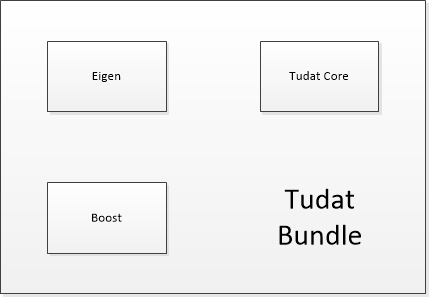
\includegraphics[width=0.3\textwidth]{figures/software/tudatBlock.png}
\caption{\ac{Tudat} structure}
\label{fig:tudatBlock}
\end{figure}

\subsection{Eigen}
\label{subsec:eigen}
Eigen is an external C++ library that was written to perform linear algebra computations \footnote{More documentation on Eigen can be found on \url{eigen.tuxfamily.org/dox/} [Accessed 8 March 2016] }. The software is free and easy to use, which is why it is widely used by the C++ community and thus also within \ac{Tudat} \citep{dirkx2016tudat}. Another advantage is that because it does not use any source files, it does not need to be build before using it. 
The Eigen libraries contain a number of standardized matrices and vectors, each with its own characteristics. An example of an often used vector is \textit{Vector3d} (or \textit{Eigen::Vector3d}), which can for instance be used to store the Cartesian position of a satellite. Here the \textit{3} shows that it can store 3 values/parameters and the \textit{d} shows that these are of the type \textit{double}. It is mentioned on the \ac{Tudat} wiki \citep{dirkx2016tudat} that these Eigen vectors and matrices should only be used if required for linear algebra computations. For ordinary storage, the C++ arrays, vectors and matrices should be used to save both storage and computation time.


\subsection{Boost}
\label{subsec:boost}
Boost is a slightly more complicated set of C++ libraries, where compared to the Eigen library, Boost first has to be compiled before being able to use all of its functionalities. Fortunately, this compiling is performed by \ac{Tudat} automatically when setting it up for the first time. Boost is described as an addition to the standard C++ libraries, thus adding more functionalities \citep{dirkx2016tudat} \footnote{More documentation on Boost can be found on \url{http://www.boost.org/} [Accessed 8 March 2016]}. Within \ac{Tudat}, Boost is used to pass free and class functions as an argument to another object and also for dynamic allocation using so-called pointers. Four libraries that are often used within \ac{Tudat} are \textit{boost::function}, \textit{boost::bind}, \textit{boost::shared\_ptr} and \textit{boost::make\_shared}. The first two libraries are used to pass functions (a function is pointed to by \textit{function} and called by \textit{bind}) and the last two are used in case of dynamic allocation (\textit{shared\_ptr} is the pointer and \textit{make\_shared} is the object creator that returns a shared pointer to the created object). 

%\subsection{\ac{PaGMO}}
%\label{subsec:pagmo}
%\ac{PaGMO} is a free optimisation tool developed by \ac{ESA}s \ac{ACT}. It uses parallel computations to perform the optimisation and can even optimise for multi-objective problems. Parallel computation is the act of performing multiple computations on the same machine using different CPU cores. This allows the cost function to be computed for different sets of optimisation parameters at the same time and thus reducing the total CPU time required. However, this only works if the cost function evaluations are independent, which is not always the case (e.g. Dynamic \ac{DE} described by \cite{qing2009differential}). The tool itself incorporates many different local and global optimisation methods as mentioned by \cite{izzo2012pygmo}, among which the optimisation method used in this thesis \ac{MBH}. This method has been written in \ac{PaGMO} in such a way that it can use any of the provided local optimisers. \ac{PaGMO} is written in C++ and requires the shared libraries of Boost to run \footnote{More documentation on \ac{PaGMO} can be found on \url{https://esa.github.io/pagmo/} [Accessed 9 March 2016]}. Interfaces to external libraries are also provided, which can incorporate for instance \ac{SNOPT} as a local optimisation method. In this thesis \ac{SNOPT} is used as the local optimiser for \ac{MBH} as implemented by \ac{PaGMO}. More information on \ac{SNOPT} is provided in \Cref{subsec:snopt}. For \ac{SNOPT} to be recognised by \ac{PaGMO}, it has to be installed separately. \Cref{fig:pagmoBlock} shows \ac{PaGMO} with the internally used Boost library and the externally called \ac{SNOPT} software.
%
%\begin{figure}[!ht]
%\centering
%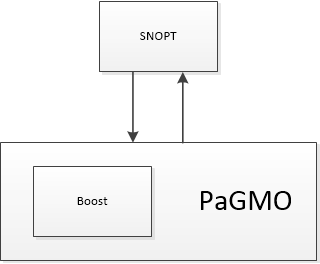
\includegraphics[width=0.3\textwidth]{figures/software/pagmoBlock.png}
%\caption{\ac{PaGMO} structure}
%\label{fig:pagmoBlock}
%\end{figure}
%
%\subsection{\ac{SNOPT}}
%\label{subsec:snopt}
%\ac{SNOPT} was introduced by \cite{gill2002snopt} as a \ac{SQP} method. It uses the first function derivatives and is very effective with highly constrained problems such as trajectory optimisation. Because it is based on \ac{SQP} it is only able to find  the local optimum and it is thus not guaranteed that this is also the global optimum. By combining \ac{SNOPT} and \ac{MBH} the global optimum can indeed be found or approached. The tool itself does not require that many evaluations, which is why it is very useful for complex problems with many optimisation variables \citep{gill2006user}. The code for \ac{SNOPT} has been written in Fortran, but can easily be translated to C,C++ using \textit{f2c} which is provided with \ac{SNOPT} as well \footnote{More documentation on \ac{SNOPT} can be found on \url{http://www.sbsi-sol-optimize.com/asp/sol_products_snopt_desc.htm} [Accessed 9 March 2016]}. This way it can be called by \ac{PaGMO}. It should be noted that \ac{SNOPT} is not free and can only be used under a licence agreement.

\subsection{Mars-\ac{GRAM}}
\label{subsec:marsgram}
Mars-\ac{GRAM} is a high-fidelity atmospheric model developed by NASA to simulate the global atmospheric conditions on Mars \citep{justus2008utilizing} \footnote{NASA website: \url{https://see.msfc.nasa.gov/model-Marsgram} [Accessed 9 March 2016]}. The model is based on NASA Ames Mars General Circulation Model (for altitudes between 0-80 km) and Mars Thermospheric General Circulation model (for altitudes above 80 km). It can provide density, temperature and pressure data (among other data) with respect to the current altitude, latitude and longitude on Mars.  Seasonal variations are taken into account in the model as well, which is why different calender dates will result in different atmospheric compositions. The tool can be used within a simulation tool or as a separate executable. Unfortunately, because it is so detailed, each computation requires a lot of CPU time. This is why it was decided to use the stand-alone Mars-\ac{GRAM} executable to generate a detailed table with atmospheric data as a function of altitude, latitude and longitude at the start of the optimisation. Even generating this table required a lot of CPU time (on average a single computation using the stand-alone executable took 67.9 seconds to complete). The starting altitude was set at -0.6 km \ac{MOLA} and advanced with a step-size of 0.1 km to 320 km altitude to cover the entire range that the \ac{MAV} would have to cover. Also, the latitude and longitude were varied within 10 degrees from the launch site with a step-size of 1 degree. A Matlab script was written to extract the relevant atmospheric data from the Mars-\ac{GRAM} output files and write them into a .csv file, thus creating the required atmospheric data table. The atmospheric data in this table was then interpolated to provide an estimate of the atmospheric characteristics at every point along the ascent trajectory, which is required to compute the drag at each time step. Some of the earlier versions of Mars-\ac{GRAM} are available for free (such as the Mars-\ac{GRAM} 2005 version used in this thesis), however, the latests versions (such as the Mars-\ac{GRAM} 2010 version used as a back-up in this thesis) require a licence agreement.


\section{Developed software}
\label{sec:developedsoftware}
This section of the software chapter describes the software that either had to be developed around existing software/libraries or had to be developed from scratch (the \ac{TSI} propagator). Each piece of software is accompanied by the corresponding software architecture. Every next piece of software then indirectly incorporates the previous architecture through the use of the completed tool.


%\subsection{Interpolator}
%\label{subsec:interpolatorsoft}
%
%\begin{figure}[!ht]
%\centering
%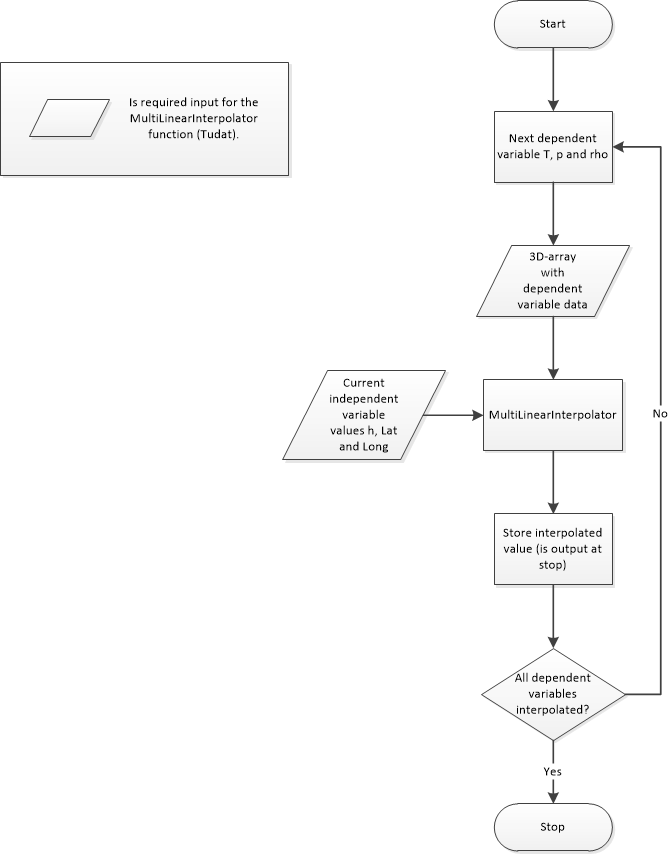
\includegraphics[width=0.5\textwidth]{figures/software/interpolator.png}
%\caption{Interpolator interface architecture}
%\label{fig:interpolator}
%\end{figure}




\subsection{\ac{RKF} propagator}
\label{subsec:rkpropagator}
The \ac{RKF} (or traditional) propagator architecture is described in \Cref{fig:RK_Propagator}. It starts with the current state, which is then passed on to the state derivative function. The state derivative function is used by the \ac{RKF} integrators to determine the next state by calling the function a number of times depending on the used method. Both \ac{RK4} and \ac{RKF45} (and higher order \ac{RKF} integrators) are already available through the \ac{Tudat} libraries. \ac{RK4} can be called by including the rungeKutta4Integrator.h header file, and \ac{RKF} methods can be called by including the rungeKuttaVariableStepSizeIntegrator.h header file. This integration process is repeated until the final condition is met. Within the state derivative function all the sate derivatives are updated and stored. The current position is used to update the gravitational acceleration on the \ac{MAV}, the current mass is used to determine the accelerations caused by the thrust and finally the complete state is required to determine the accelerations caused by the drag. Both the drag and thrust accelerations have to be transformed to the inertial frame using the updated angles from the current state. The function also computes the current mass flow rate, however since the thrust is constant, this does not change over time. In the state derivative function, all the transformations are governed by pre-developed functions within the \ac{Tudat} library, which includes the state transformations and the frame transformation from the body frame to the inertial frame. The transformation from the propulsion frame to the body frame is however not included in \ac{Tudat} and had to be written.


\begin{figure}[!ht]
\centering
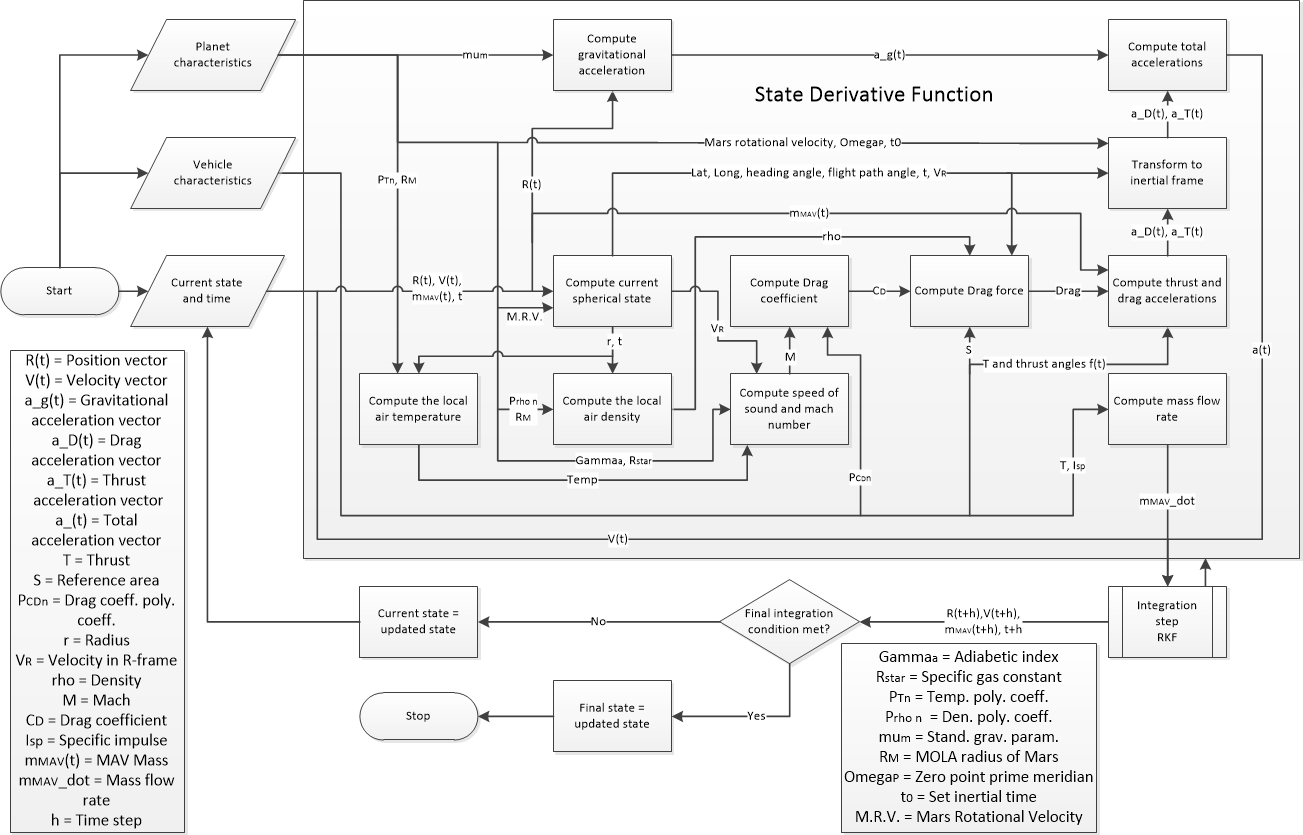
\includegraphics[width=1.5\textwidth, angle = 90]{figures/software/RK_Propagator.png}
\caption{\ac{RKF} interface architecture}
\label{fig:RK_Propagator}
\end{figure}

All blocks represent a different action. These actions might be performed in classes, header files and/or source files. More information on the classification of the different blocks can be found in \Cref{app:appendixC-programFileDefinitions}.

\subsection{\ac{TSI} propagator}
\label{subsec:tsipropagator}
The \ac{TSI} propagator has a significantly different architecture compared to the traditional propagator as can be seen in \Cref{fig:TSI_Propagator}. \ac{TSI} requires an initial order and step-size to start the integration process. In this thesis it has been decided to keep the order the same throughout the entire integration. The step-size will change during the integration depending on the Taylor series evaluations. The initial state is set as the current state and is fed into the \ac{TSI} block. Within this block, first the auxiliary equations and functions are called, which were set-up for this particular problem. They are evaluated using the current state. These auxiliary equations and functions already include all the reference frame and coordinate transformations, as well as approximate atmospheric parameter functions. This is required to set-up the recurrence relations, which is where \ac{TSI} differs from the traditional propagator. Once the auxiliary equations and functions have been computed they are used to compute the Taylor coefficients through the recurrence relations set-up for the thesis problem. These coefficients are then stored for later use and are also passed to the block creating the Taylor series expansion for every state variable thus creating the updated state. The last two coefficients are then used to determine the next step-size. This continues until the final integration condition has been met. 


\begin{figure}[!ht]
\centering
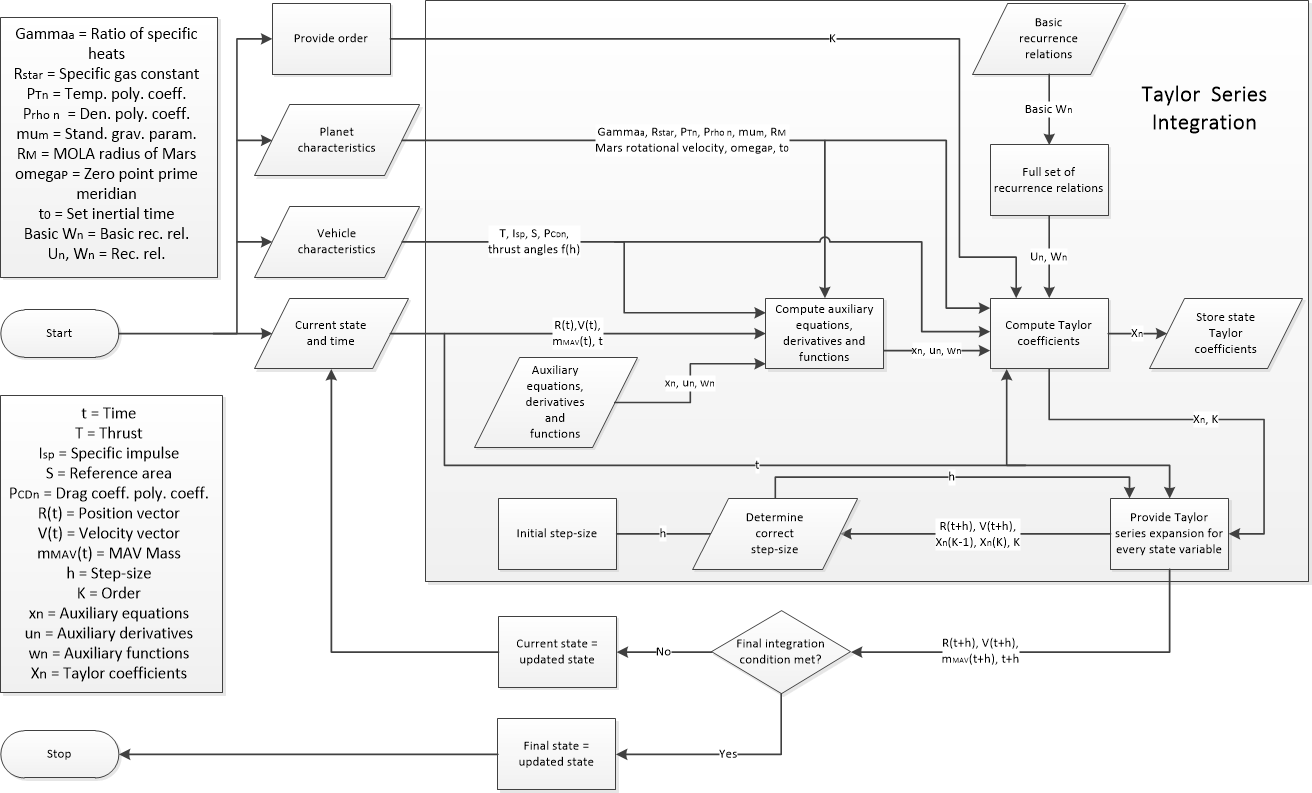
\includegraphics[width=1.5\textwidth, angle = 90]{figures/software/TSI_Propagator.png}
\caption{\ac{TSI} architecture}
\label{fig:TSI_Propagator}
\end{figure}


%\subsection{Optimiser}
%\label{subsec:optimisersoft}
%The optimisation software is a combination of the \ac{SNOPT} local optimisation tool and \ac{PaGMO}s \ac{MBH}. Even though both these tools were already available and did not have to be developed, it is still important to understand how the rest of the software interacts with the optimiser. This is why  \Cref{fig:optimiser} shows the architecture of the \ac{MBH} optimiser. It starts with the initial generation of the optimisation parameters, after which the 'Number of not improved iterations' is set to zero. This is then fed into the local optimiser, where the trajectory is integrated using the previously described tools. Once a local optimised trajectory is found, it is stored if it is better than the previous local optimised trajectory and the counter is set to zero again. If the newly found trajectory is not better than the current best the 'Number of not improved iterations' is increased by one. Once the maximum number of not improved iterations is met, the current best optimal trajectory (which is the optimum for the current "funnel") is stored and the process is repeated till the final global optimisation condition is met. At this point the global optimum is the best optimal trajectory from all the funnels computed at that time, which is then returned as the program solution.
%
%\begin{figure}[!ht]
%\centering
%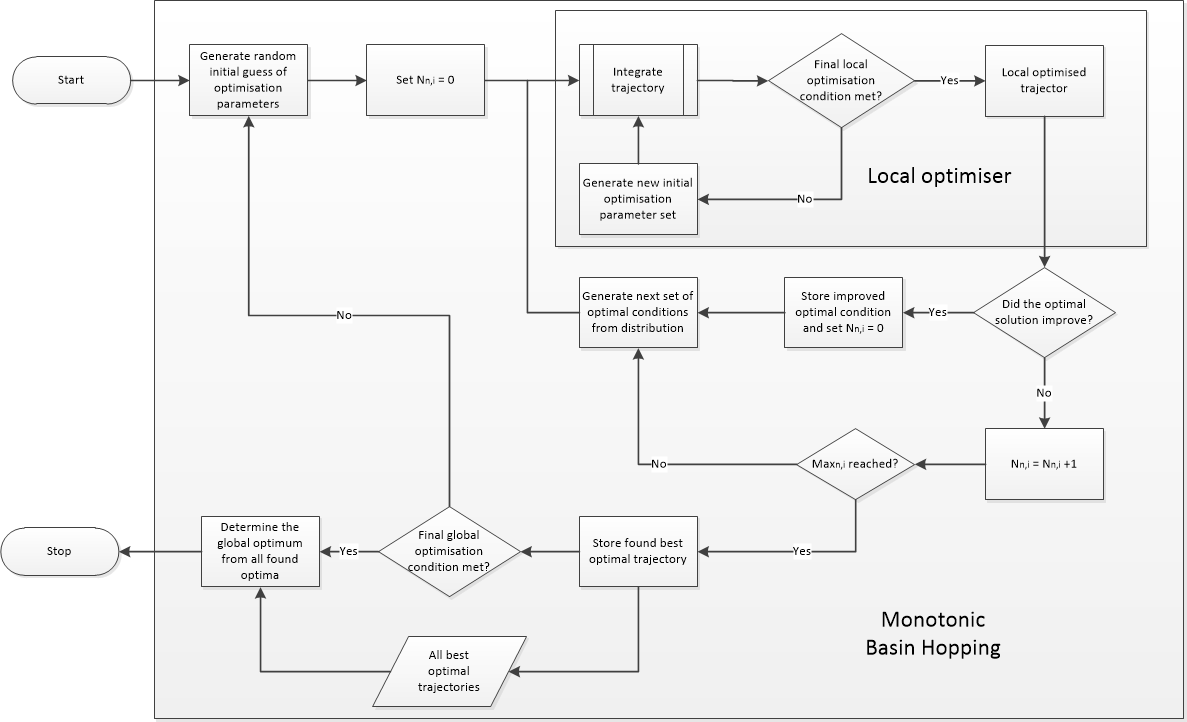
\includegraphics[width=1.5\textwidth, angle = 90]{figures/software/optimiser.png}
%\caption{Optimiser interface architecture}
%\label{fig:optimiser}
%\end{figure}

\section{Completed simulation tool}
\label{sec:completedSimulationTool}
The final simulation tool combined the integration software in such a way that a complete trajectory propagation could be simulated. It consists of different phases: initialisation, initial propagation, integrator burn phase, integrator coast phase, final circularisation and comparison. A brief description of each phase is provided in this section. It should be noted that in the actual program, the \ac{TSI} propagation (burn and coast phase) supersedes the \ac{RKF} propagation. Also, three different \ac{RKF} methods can be chosen: \acf{RKF45}, \ac{RKF78} and  \ac{DOPRIN87}.

\subsection{Initialisation}
\label{subsec:initialisation}
During the initialisation phase, all the input values are loaded into the program. This is done by calling the input .txt files and assigning all the proper values to the corresponding parameters. Then, the Mars celestial body class and the \ac{MAV} class are initialised, providing the Mars atmospheric and planetary data and the \ac{MAV} system characteristics respectively. At this point, any values that differ from the pre-set default values are updated in both classes. The next step is to convert the initial spherical state into the initial Cartesian state and both states are saved in the respective output files for both \ac{TSI} and \ac{RKF}. Finally, the StateAndTime class is initialised for the \ac{TSI}.

\subsection{Initial propagation}
\label{subsec:initialPropagation}
As will be described in \Cref{ch:verificationandvalidation}, during the verification process it was found that \ac{TSI} had trouble dealing with initial conditions close to its singular values during the initial second(s), both for velocity and flight-path angle. This is why it was decided to slightly shift the initial conditions at which the actual integration for \ac{TSI} would start. Because \ac{RKF} did not have similar issues with the first second(s), it was chosen to use an \ac{RKF} method to propagate the first second. For this initial integration, the default integrator is \ac{RKF78} with a tolerance of $1\cdot 10^{-15}$. The output of this initial propagation is then used as the initial state for both \ac{TSI} and \ac{RKF} for the remainder of the integration. This way, both methods can still be compared properly. 


\subsection{Integrator burn phase}
\label{subsec:integratorBurnPhase}
At the start of the burn phase the final state of the initial propagation is taken as the initial state input for the integrators. During the burn phase, both \ac{TSI} and \ac{RKF} are initiated and run until the end of the first burn phase occurs. Within this phase, \ac{TSI} stops at every altitude and Mach section of the atmospheric graphs to make sure that no errors occur in the model. Provided that the atmospheric graphs are piecewise continuous, such stops are not required for \ac{RKF}. The end of the first burn phase can either be based on a set time or a set altitude. Of course, extra cut-off criteria can be added. During the propagation, all intermediate states are stored in the output files for both methods.


\subsection{Integrator coast phase}
\label{subsec:integratorCoastPhase}
After the first burn phase, the \ac{MAV} enters a coasting phase. This is simulated by setting the thrust equal to zero. For \ac{TSI} this can simply be done by setting the thrust in the \ac{MAV} class zero within the propagation do-loop. This means that when the set burn-out condition is met, the class is updated, and the loop is continued. However, it is not possible to do this within one loop for the \ac{RKF}, because of the manner in which \ac{RKF} is initialised. In \ac{Tudat} it is described that in order to use the build in \ac{RKF} functions, a separate state derivative class has to be build first. This class is initialised using the initial state classes, and therefore does not change when updating the initial state classes in the loop directly. This means that when the thrust changes to zero, the state derivative class has to be re-initialised, creating the need for a second separate do-loop. This also means that the integrator class has to be re-initialised as well, which means that a separate integrator has to be defined (one with a different name from the first one). Both the \ac{TSI} and \ac{RKF} coasting phases are terminated whenever the desired altitude is reached, or after a certain limit time. Again, all the intermediate states are stored in the output files during the coasting phase.


\subsection{Final circularisation}
\label{subsec:finalCircularisation}
Once the final condition is met, both the \ac{RKF} and the \ac{TSI} final state are used to determine the required final circularisation burn in order to reach the desired final orbit. For this computation, the states are first converted into Kepler elements using the \ac{Tudat} library. Then the required $\Delta V$ is computed using the methods described by \cite{wakker2010}. In this case, an instantaneous burn to change the inclination, flight-path angle and orbital velocity to match the desired orbit is assumed. From the $\Delta V$ for both methods, it can be determined, using   the Tsiolkovsky rocket equation what the required propellant mass is. This then results in a final mass estimate for both the \ac{RKF} and the \ac{TSI} propagations.


\subsection{Comparison}
\label{subsec:comparison}
Finally, the end states of both \ac{TSI} and \ac{RKF} are compared to each other. The program provides the numeric difference between the position, velocity and mass as well as the quotient between those values. This quotient, or difference fraction, is the \ac{TSI} state divided by the \ac{RKF} state and the numeric difference is the \ac{TSI} state minus the \ac{RKF} state. These values were used in the verification and validation phase and are used during the thesis analysis as well to show the behaviour of \ac{TSI} compared to \ac{RKF}.  


%\section{Architectures}
%\label{sec:architecture}